\documentclass[12pt, letterpaper]{article}

\setlength{\topmargin}{-1.75cm} \setlength{\textheight}{22.5cm}
\setlength{\oddsidemargin}{0.25cm}
\setlength{\evensidemargin}{0.25cm} \setlength{\textwidth}{16.2cm}
\renewcommand{\figurename}{Figure}
\usepackage{amssymb}
\usepackage{graphicx}
\usepackage{amsmath}
\usepackage[normalem]{ulem}
\usepackage{fontenc}
\usepackage{hyperref}
\usepackage{footnote}

\usepackage{palatino, url, multicol, listings} % for multiple columns
\lstset{mathescape=true, basicstyle=\ttfamily,}

%\usepackage{pictex}
%% in the .pictex output of xfig, there is command \colo
%% however the old version of pictex may not define this
%% so we define color here as empty
%\def \color#1]#2{}

\begin{document}

\newcommand{\hide}[1]{}
\newcommand{\exercise}[1]{}
\newcommand{\future}[1]{}
\newcommand{\otherquestions}[1]{}
\newcommand{\set}[1]{\{#1\}}
\newcommand{\pg}[1]{{\tt #1}}
\newtheorem{definition}{Definition}
\newcommand{\emptyclause}{\Box}
\def\st{\bigskip\noindent}
\newcommand{\lplus}
{
   \stackrel{+}{\gets}
}

\newcommand{\fe}[1] {
  \begin{frame}
    #1
  \end{frame}}

\newcommand{\eoa}{ {\bf End} of algorithm}

\newcommand{\ft}[1] {\frametitle{#1}}

\newcommand{\ie}[1] {
  \begin{itemize}
    #1
  \end{itemize}
}

\newcommand{\ee}[1] {
  \begin{enumerate}
    #1
  \end{enumerate}\label{marker}
}
\newcommand{\blk}[2] {
  \begin{block}{#1}
    #2
  \end{block}
}

\newtheorem{collorary}{Corollary}
\newtheorem{proposition}{Proposition}
\newtheorem{invariant}{Invariant}
\newtheorem{property}{Property}
\newtheorem{claim}{Claim}
\newtheorem{example}{Example}


\title{${\cal SPARC}$ manual}
\date{\today}
\maketitle
\tableofcontents
\pagebreak


\section{System installation}

\st For using the system, you need to have the following installed:
\begin{enumerate}
\item Java Runtime Environment (JRE) can be found here \url{http://www.oracle.com/technetwork/java/javase/downloads/index.html}.
The system was tested on Java versions 1.6.0\_37 and 1.7.0\_25.
\item The SPARC to ASP translator. It can be downloaded here: \url{https://github.com/iensen/sparc/blob/master/sparc.jar?raw=true}.
\item An ASP solver. It can be one of the following:
\begin{enumerate} 
\item DLV (recommended).
 \url{http://www.dlvsystem.com/dlv/#1}You need to download the \textit{static} version of the executable file.
\item Clingo \url{http://sourceforge.net/projects/potassco/files/clingo/3.0.5/}.
\end{enumerate}

\item (\textit{optional}) Swi-Prolog. \url{http://www.swi-prolog.org/}. This item is only required if option \textit{-wcon} is used for type warning detection.
(See sections \ref{option} and \ref{clp_type_warnings}).

\end{enumerate}
If you are using dlv solver, rename the solver executable file to \textit{dlv} (\textit{dlv.exe} for windows).
Make sure the solver you are using is in your system \texttt{PATH} variable (see figures \ref{fig:dlv_solver_check} for dlv and \ref{fig:clingo_solver_check} for clingo).

\begin{figure}[p]
\centering
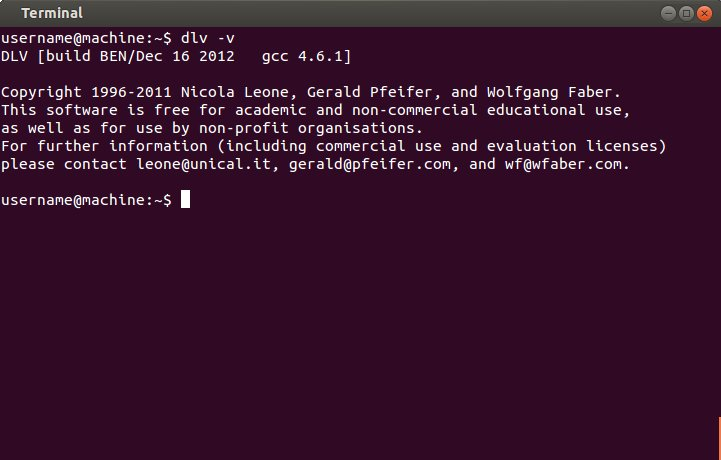
\includegraphics[width=0.9\textwidth]{dlv_version.jpg}
\caption{Checking the version of DLV solver}
\label{fig:dlv_solver_check}
\end{figure}


\begin{figure}[p]
\centering
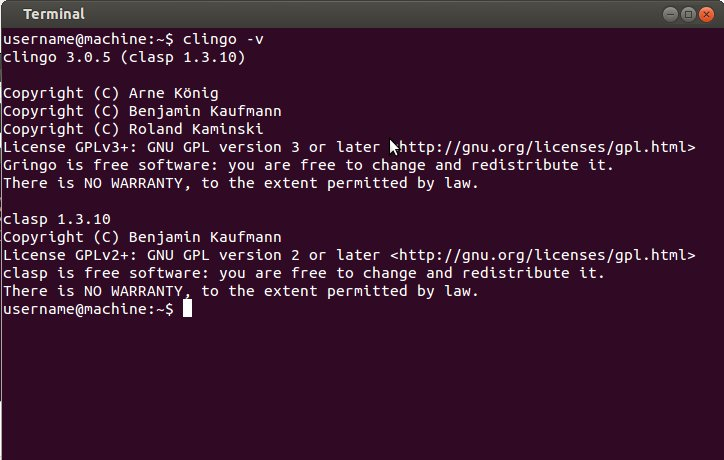
\includegraphics[width=0.9\textwidth]{clingo_version.jpg}
\caption{Checking the version of Clingo solver}
\label{fig:clingo_solver_check}
\end{figure}

\section{System usage}

To demonstrate the usage of the system we will use the program $\Pi$ below.
\begin{verbatim}
sorts
#person={bob,tim,andy}.
predicates
teacher(#person).
rules
teacher(bob).
\end{verbatim}

\st
The system can work in one of the  two modes: \textit{querying mode} and \textit{answer set mode}.

\subsection{Querying mode}

In this mode we can ask queries about a ${\cal SPARC}$ program loaded into the system.
The general command line syntax for this mode is \textit{java -jar sparc.jar program\_file}.
Queries in ${\cal SPARC}$ are positive or negative literals of the forms $p(t1,t2,\dots,tn)$ or
$-p(t1,t2,\dots,tn)$ correspondingly, where $p(t1,t2,\dots,tn)$  is an atom of the loaded program $\Pi$ 
( note that \textit{n} can be equal to zero, in this case the query will be of the form \textit{p} or \textit{-p}  ).

The queries are answered as follows:
\ie{
\item The answer to a query $l$ not containing variables is \textit{yes}, if $l$(with all arithmetic expressions evaluated) belongs to all answer sets of  $\Pi$.
\item The answer to a query $l$ not containing variables is \textit{no}, if $-l$(with double classical negation removed and all arithmetic expressions evaluated) belongs to all answer sets of  $\Pi$.
\item The answer to a query $l$ not containing variables is \textit{unknown}, if it is not \textit{yes} or \textit{no}.
\item The answer to a query of the form $l$($l$ is an atom of the form $p(t1, \dots, tn)$  possibly preceeded by a negation sign)  is  a collection of assignments $X_1 = t_1, \dots, X_n=t_n$,
where $X_1, \dots, X_n$ are all variables in $p(t1, \dots, tn)$, $t_1, \dots, t_n$ are ground terms, and the answer to the query $p(t1',\dots,tn')$, obtained from  $p(t1, \dots, tn)$ by replacing each variable $X_i$ by a ground term $t_i$, is \textit{yes}.

}
 
For the program $\Pi$ above, written in the file \texttt{program.sp}, we run the queries shown below. 

\begin{verbatim}
username@machine:~$ java -jar sparc.jar program.sp
SPARC  V2.25
program translated
?- teacher(bob).
yes
?- teacher(tim).
unknown
?- teacher(X).
X = bob
?- teacher(john).
program.sp: argument number 1 of predicate teacher/1, "john", 
            violates definition of sort "person"
?-exit.
\end{verbatim}

The answer to the first query \texttt{?- teacher(bob)} is \textit{yes}, because the atom \textit{teacher(bob)} belongs to the only answer set of $\Pi$.

The answer to the second query \texttt{?- teacher(tim)} is \textit{unknown}, because neither the atom \textit{teacher(bob)} nor its negation belongs to the answer set of $\Pi$.

The answer to the query \texttt{?- teacher(X)} is \textit{X = bob}, because there is only one replacement (bob) for X, such that \textit{teacher(X)} belongs to the answer set of $\Pi$.

For the fourth query, we see an error, because teacher(john) is not an atom of $\Pi$.

To quit the querying engine, use \textbf{exit} command.

\subsection{Answer Set Mode}

In this mode we can see the computed answer sets of the loaded program.
The general command line syntax for this mode is \textit{java -jar sparc.jar program\_file -A}.

For the program $\Pi$, the answer set may be computed as it is shown below:
\begin{verbatim}
username@machine:~$ java -jar sparc.jar program.sp -A
SPARC  V2.25
program translated
DLV [build BEN/Dec 16 2012   gcc 4.6.1]
{teacher(bob)}

\end{verbatim}

\section{Command Line Options}\label{option}

In this section we  describe the meanings of command line options supported by
${\cal SPARC}$. Some options(flags) do not take an argument and have the form \textit{-option},
while others require arguments and can be written in the form \textit{-option arg}.
For each command line option, we indicate whether it requires
an argument, and if so, we  describe its meaning.

\begin{itemize}
 \item \textbf{-A}
    
  Compute answer sets of the loaded program.

\item \textbf{-wcon}
    
  Show warnings determined by CLP-based algorithm. See section \ref{clp_type_warnings}

\item \textbf{-wasp}
    
  Show warnings determined by ASP-based algorithm. See section \ref{asp_type_warnings}

\item \textbf{-solver arg}

  Specify the solver which will be used for computing answer sets. \textit{arg} can have two possible values: \textit{dlv} and \textit{clingo}. 
\item \textbf{-solveropts arg}

  Pass command line arguments to the ASP solver (DLV or Clingo).
  
  Example: \texttt{-solveropts "-pfilter=p"}.


  For the complete list of dlv options, see 
  \url{http://www.dlvsystem.com/html/DLV_User_Manual.html }


  For the complete list of clingo options, see 
  \url{http://sourceforge.net/projects/potassco/files/potassco_guide/}

  Note that options "0" and "--shift" are passed to clingo solver by default.

\item \textbf{-Help, -H, -help, --Help, --help, -h}

  Show help message.

\item \textbf{-o arg}

  Specify the output file where the translated ASP program will be written. \textit{arg} is the path to the output file. 
  Note that if the option is not specified, the translated ASP program will not be stored anywhere.

\item \textbf{input\_file}
  
Specify the file where the sparc program is located.



\end{itemize}


\section{Syntax Description}

\subsection{Directives}
Directives should be written before sort definitions, at the very beginning of a program.
${\cal SPARC}$ allows two types of directives:
\subsection*{\#maxint}
Directive \#maxint specifies maximal nonnegative number which could be used in arithmetic calculations. For example,
\begin{verbatim}
 #maxint=15.
\end{verbatim}
\st limits integers to [0,15].
\subsection*{\#const}
Directive \#const allows one to define constant values. The syntax is:
\begin{verbatim}
   #const constantName = constantValue.
\end{verbatim}      
\st where $constantName$  must begin with a lowercase letter and may be composed of letters, underscores and digits,
 and $constantValue$ is either a nonnegative number or the name of another constant defined above.  


\subsection{Sort definitions}\label{ss}

This section starts with a keyword $sorts$ followed by a collection of sort definitions of the form:

\begin{verbatim}
  sort_name=sort_expression.
\end{verbatim}

The sort expression on the right hand side denotes collection of strings called $sorts$. We divide all the sorts into \textit{basic} and \textit{non-basic}. 

\st \textit{Basic sorts} are defined as named collections of identifiers, i.e, strings consisting of
\begin{itemize}
 \item latin letters: $\{a,b,c,d,...,z,A,B,C,D,...,Z\}$
 \item digits: $\{0,1,2,...,9\}$
 \item underscore: $\_$
\end{itemize}
and either starting from a letter or containing only digits.

Non-basic sorts also contain \textit{records} of the form $id(\alpha_1,\dots, \alpha_2)$, where id is an identifier and 
$\alpha_1, \dots, \alpha_n$ are either identifiers or records. 


\st We define sorts by means of expressions(in what follows sometimes referred as statements) of five types:

\begin{enumerate}
 \item \textbf{set-theoretic expression}.
 \begin{verbatim}
  set_expression := #sort_name | {ground_term_list}
  set_expression := (set_expression) 
                    | (set_expression + set_expression ) 
                    | (set_expression * set_expression ) 
                    | (set_expression - set_expression )
  \end{verbatim}
The operations $+$ $*$ and $-$ stand for union, intersection and difference correspondingly.
\texttt{ground\_term\_list} is set of \textit{ground terms}, defined as follows:
\begin{itemize}
 \item numbers and constants are ground terms;
 \item If $f$ is an identifier and $\alpha_1, \dots, \alpha_n$ are ground terms, then $f(\alpha_1,\dots, \alpha_n)$ is a ground term.
\end{itemize}
\textit{Example} : 
\begin{verbatim}
 sort1={f(a),a,b,2}.
 sort2={1,2,3} + {a,b,f(c)} -  {f(a),a,b,2}.
\end{verbatim}
According to the definition, \texttt{sort1} consists of ground terms $\{f(a),a,b,2\}$, and \texttt{sort2} is $\{1,2,3,f(c)\}$ 

\item \textbf{numeric range}.
\begin{verbatim}
 numeric_range := number1 .. number2
\end{verbatim}

\textit{number1} should be smaller or equal than \textit{number2}. The expression defines the set 
of subsequent numbers $\{number1, number1+1, \dots, number2\}$

\textit{Example:}

\begin{verbatim}
 sort1=1..3
\end{verbatim}
\texttt{sort1} consists of numbers $\{1,2,3\}$.


\item \textbf{identifier range}


\begin{verbatim}
 id_range := id1 .. id2
\end{verbatim}

\textit{id1} should be lexicographically smaller or equal than \textit{id2}. 
\textit{id1} and \textit{id2} should both consist of digits and letters.
The expression defines the set of all strings \\ S=$\{s: id1\leq s \leq id2 \land |id1|\leq |s| \leq |id2|\}$



\textit{Example:}

\begin{verbatim}
 sort1=a..f.
\end{verbatim}
\texttt{sort1} consists of latin letters $\{a,b,c,d,e,f\}$.

\item \textbf{concatenation}
\begin{verbatim}
concatenation := [b_stmt_1] ... [b_stmt_n]
\end{verbatim}

\texttt{b\_stmt\_1}, $\dots$, \texttt{b\_stmt\_n} must be \textit{basic statements}, defined as follows:


\begin{itemize}
 \item statements of the forms (2)-(4) are basic
 \item statement $S$ of the form (1) is basic if:
 \begin{itemize}
  \item all curly brackets occurring in $S$ contain only constants consisting of latin letters and digits
  \item all sorts occurring in $S$ are defined by basic statements 
 \end{itemize}
\end{itemize}
Note that basic statement can only define a basic sort not containing records.

\textit{Example\footnote{We allow a shorthand `b` for singleton  set \{b\}}.:}

\begin{verbatim}
 sort1=[b][1..100].
\end{verbatim}

\texttt{sort1} consists of identifiers $\{b1,b2,\dots, b100\}$.


\item \textbf{record}


\begin{verbatim}
 functional_term := f(sort_name1(var_1),..., sort_namen(var_n)):
                                     condition(var_1,...,var_n)
 condition(var_1,...,var_n) := var_i REL var_j 
 condition(var_1,...,var_n) :=   condition and condition 
              | condition or condition 
              | not(condition) 
              | (condition)
\end{verbatim}
Variables \texttt{var\_1,...,var\_n} are optional.
Condition can only contain variables from the list \texttt{var\_1,...,var\_n}.
If there is a subcondion \texttt{var\_i REL var\_j}, where REL is either $\{>,\geq,<,\leq\}$ then \texttt{sortname\_i} and then \texttt{sortname\_j}
must be defined by basic statements.

The expression defines a collection of ground terms 
\\ $\{f(t_1,\dots,t_n): condition(t_1,\dots, t_n)~is~true \land t_1 \in s_i \land \dots \land t_n \in s_n\}$

\textit{Example}
\begin{verbatim}
 #s=1..2.
 #sf=f(s(X),s(Y),s(Z)): (X=Y or Y=Z). 
\end{verbatim}

The sort \texttt{sf} consists of records $\{f(1,1,2),f(1,1,1),f(2,1,1)\}$

\end{enumerate}

\subsection{Predicate Declarations}

\noindent  The second part of a  ${\cal SPARC}$ program starts with the keyword
\st
$predicates$

\st and is followed by statements of the form

\st
$pred\_symbol(sortName,\dots,sortName)$

\st

Multiple declarations containing the same predicate symbol are not allowed.
0-arity predicates must be declared as $pred\_symbol()$.
\st For any sort name $SN$, the system includes declaration  $SN(SN)$ automatically.

\subsection{Program Rules}


\st The third part of a ${\cal SPARC}$ program starts with the keyword \textit{rules} followed by standard ASP rules(supported by the specified ASP solver\footnote{Currently, only DLV solver is fully supported(excluding \#import directives). Clingo's choice rules and minimize statements will be added later}) and/or consistency restoring (cr)-rules.
\st
CR-rules are of the following form:

\begin{equation}
   [label:] l_0 \lplus l_1,  \ldots, l_k, not~l_{k+1} \ldots not~l_{n}
 \end{equation}
where $l$'s are literals.
Literals occurring in the heads of the rules must not be formed by predicate symbols
occurring as sort names in sort definitions. In addition, rules must not contain \textit{unrestricted variables}.

\begin{definition}(Unrestricted Variable)
 A variable occurrung in a rule of a ${\cal SPARC}$ program is called unrestriced if all its occurrences in the rule either belong to some relational atoms of the form 
$term1$ \textbf{rel} $term2$ (where \textbf{rel} $\in  \{>,>=,<,<=,=,!=$\})  and/or  some terms appearing in a head of a choice or aggregate element. 
\end{definition}
\begin{example}
\em{
 Consider the following ${\cal SPARC}$ program:
\begin{verbatim}
sorts
#s={f(a),b}.
predicates
p(#s).
rules
p(f(X)):-Y<2,2=Z,F>3,#count{Q:Q<W,p(W),T<2},p(Y).
\end{verbatim}
Variables F,T,Z,Q are unrestricted.
}  
\end{example}

 
\section{Answer Sets}
\noindent A set of ground literals $S$ is an {\em answer set} of a ${\cal SPARC}$ 
program $\Pi$ with regular rules only if $S$ is an answer set of an ASP program consisting of the same rules.

\st To define the semantics of a general ${\cal SPARC}$ program, we need notation for abductive support.
By $\alpha(r)$ we denote a regular rule
obtained from a consistency restoring rule $r$
by replacing $\lplus$ by $\leftarrow$;
$\alpha$ is expanded in the standard way to a set $X$ of CR-rules,
i.e., $\alpha(A) = \{\alpha(r)\; :\; r \in A\}$.
\st A %minimal (with respect to the preference relation $\leq$ of the program)
collection $A$ of CR-rules of $\Pi$ such that
\begin{enumerate}
\item $R \cup \alpha(X)$ is consistent (i.e., has an answer set), and
\item any $R_0$ satisfying the above condition has cardinality
which is greater than or equal to that of $R$
\end{enumerate}
is called an {\em abductive support} of $\Pi$.
\st A set of ground literals $S$ is an {\em answer set} of a ${\cal SPARC}$ program 
$\Pi$ if $S$ is an answer set of $R \cup \alpha(A)$, where $R$ is the set of regular rules of $\Pi$, for some abductive
support $A$ of $\Pi$.

\st \textbf{Example}
\begin{verbatim}
sorts
#s1={a}.  % term "a" has sort "s1"

predicates
p(#s1).  %predicate  "p" accepts terms of sort s1 
q(#s1).  %predicate  "q" accepts terms of sort s1 

rules
p(a) :- not q(a).
-p(a).
q(a):+.  % this is a CR-RULE. 
\end{verbatim}
\st Result:
\begin{verbatim}
username@machine:~$ java -jar sparc.jar program -A
SPARC  V2.25
program translated
DLV [build BEN/Dec 16 2012   gcc 4.6.1]

Best model: {-p(a), appl(r_0), q(a)}
Cost ([Weight:Level]): <[1:1]>
\end{verbatim}

\st Additional literal $appl(r_0)$ was added to the answer set, which means that the 
first cr-rule from the program was applied.

\section{Typechecking}
If no syntax errors, are found,  a static check program is performed all found type-related problems, classified into type errors and type errors.
\subsection{Type errors}
Type errors are considered as serious issues which make it  impossible to complied and execute the program.
Type errors can occur in all four section of a ${\cal SPARC}$ program.
\subsubsection{Sort definition errors}
\begin{enumerate}
\item  Set-theoretic expression (statement (2) in section \ref{ss}) contains a name of undefined sort.

\textit{Example:}
\begin{verbatim}
 sorts
 #s={a}.
 #s2=#s1-s.
\end{verbatim}

\item  Sort with the same name is defined more than once.
\textit{Example:}
\begin{verbatim}
 sorts
 #s={a}.
 #s={b}.
\end{verbatim}


\item In an identifier range id1.. id2 (statement (2) in section \ref{ss}) the first identifier(id1) is lexicographically greater than id2.
\textit{Example}
\begin{verbatim}
 sorts
 #s=zbc..cbz.
\end{verbatim}

\item In a numeric range $n1..n2$ (statement (2) in section \ref{ss})  n1 is greater than n2.
\textit{Example:}
\begin{verbatim}
 sorts
 #s=100500..1.
\end{verbatim}


\item Numeric range (statement (2) in section \ref{ss}) $n1..n2$  contains an undefined constant.

\begin{verbatim}
 #const n1=5.
 sorts
 #s=n1..n2.
\end{verbatim}

\item In an identifier range $id1..id2$ (statement (3) in section \ref{ss})  the length of the first identifier(id1) is greater than length of the second. 


\textit{Example:}
\begin{verbatim}
 sorts
 #s=abc..a.
\end{verbatim}

\item Concatenation (statement  (4) in section \ref{ss}) contains a non-basic sort.

\textit{Example:}
\begin{verbatim}
 sorts
 #s={f(a)}.
 #sc=[a][#s].
\end{verbatim}



\item Record definition (statement (5) in section \ref{ss}) contains an undefined sort.

\textit{Example:}
\begin{verbatim}
 sorts
 #s=1..2.
 #fs=f(s,s2).
\end{verbatim}



\item Definition of record (statement (5) in section \ref{ss}) contains a condition with relation $>,<,\geq,\leq$ such that the
   corresponding sorts are not basic.
\textit{Example:}
\begin{verbatim}
#s={a,b}.
#s1=f(#s). 
#s2=g(s1(X),s2(Y)):X>Y.
\end{verbatim}

\item  Variable is used more than once in record definition(statement  (5) in section \ref{ss}).

\textit{Example:}

\begin{verbatim}
 sorts
 #s1={a}.
 #s=f(#s1(X),#s1(X)):(X!=X).
\end{verbatim}
\item Sort contains an empty collection of ground terms.

\textit{Example}
\begin{verbatim}
 sorts
 #s1={a,b,c}
 #s=#s1-{a,b,c}.
\end{verbatim}
\end{enumerate}
\subsubsection{Predicate declarations errors}

\begin{enumerate}
\item A predicate with the same name is defined more than once.
\textit{Example:}
\begin{verbatim}
 sorts
 #s={a}.
 predicates
 p(#s).
 p(#s,#s).
\end{verbatim}
\item A predicate declaration contains an undefined sort.
\textit{Example:}
\begin{verbatim}
 sorts
 #s={a}.
 predicates
 p(#ss).
\end{verbatim}
\end{enumerate}
\subsubsection{Program rules errors}

In program rules we first check each atom of the form $p(t_1,\dots,t_n)$ and each term occurring in the program $\Pi$ for satisfying
the definitions of program atom and program term correspondingly(!!add reference as soon as it is available). Moreover, we check that no sort occurs in a head of a rule of $\Pi$.
\subsection{Type warnings}\label{type_warnings}
During this phase each rule in input ${\cal SPARC}$ program is checked for having at least one ground instance. This is done by applying a standard constraint
satisfaction algorithm to a constraint formula over finite domains[9] produced by algorithms from (!!! add link as soon as it is available).
Warnings are reported for the rules which have no ground instances.
\subsubsection{ASP based warning checking} \label{asp_type_warnings}
The option \texttt{-wasp} must be passed to the  system  in order to detect and display warnings using a simple ASP based algorithm.
For example, consider the ${\cal SPARC}$ program below.

\begin{verbatim}
sorts
#s1={a}.
#s2=f(#s1).
#s3={b}.

predicates
p(#s2).
q(#s3).

rules
p(f(X)):-q(X).
\end{verbatim}

The only rule of the program has no ground instances with respect to defined sorts.
The execution trace is provided below
\begin{verbatim}
username@machine:~$ java -jar sparc.jar program.sp -A -wasp
SPARC  V2.25
program translated
DLV [build BEN/Dec 16 2012   gcc 4.6.1]

{s3(b), s2(f(a)), warning("p(f(X)):-q(X). ( line: 11, column: 1)")}
\end{verbatim}

The atom \texttt{warning("p(f(X)):-q(X). ( line: 11, column: 1)")} is included into the answer set as an indicator of potential problem.
When the \texttt{-wasp} is passed to ${\cal SPARC}$ system, each answer set will contain 
\begin{verbatim}
warning("rule description") 
\end{verbatim}
for each rule which has no ground instances\footnote{in current version, aggregates are skipped by this algorithm} and 
\begin{verbatim}
has_ground_instance("rule description")
\end{verbatim}
\st
for all other rules of the input program.
\subsubsection{Constraint solver based warning checking}\label{clp_type_warnings}

The option \texttt{-wcon} must be passed to the  system  in order to detect and display warnings using the algorithm described in the paper \cite{?} (!add citation as soon as it is available).
Consider the same ${\cal SPARC}$ program as above.

\begin{verbatim}
sorts
#s1={a}.
#s2=f(#s1).
#s3={b}.

predicates
p(#s2).
q(#s3).

rules
p(f(X)):-q(X).
\end{verbatim}

The only rule of the program has no ground instances with respect to defined sorts.
The execution trace is provided below
\begin{verbatim}
username@machine:~$ java -jar sparc.jar program.sp -A -wcon
SPARC  V2.25
WARNING: Rule p(f(X)):-q(X). at line 11, column 1 is an empty rule
program translated
DLV [build BEN/Dec 16 2012   gcc 4.6.1]
{s3(b), s2(f(a))}
\end{verbatim}

The message \texttt{WARNING: Rule p(f(X)):-q(X). at line 9, column 1 is an empty rule} is an indicator of a potential problem.

\section{${\cal SPARC}$ and ASPIDE}
For using ${\cal SPARC}$ in ASPIDE, you will need to install ASPIDE version 1.37.1 or greater. Once it is install, go to \textit{File -\textgreater Plug-ins -\textgreater Available plugins} menu, 
and press install button in the row containing ${\cal SPARC}$ plug-in (see Fig.\ref{fig:plug_install}).
\begin{figure}[p]
\centering
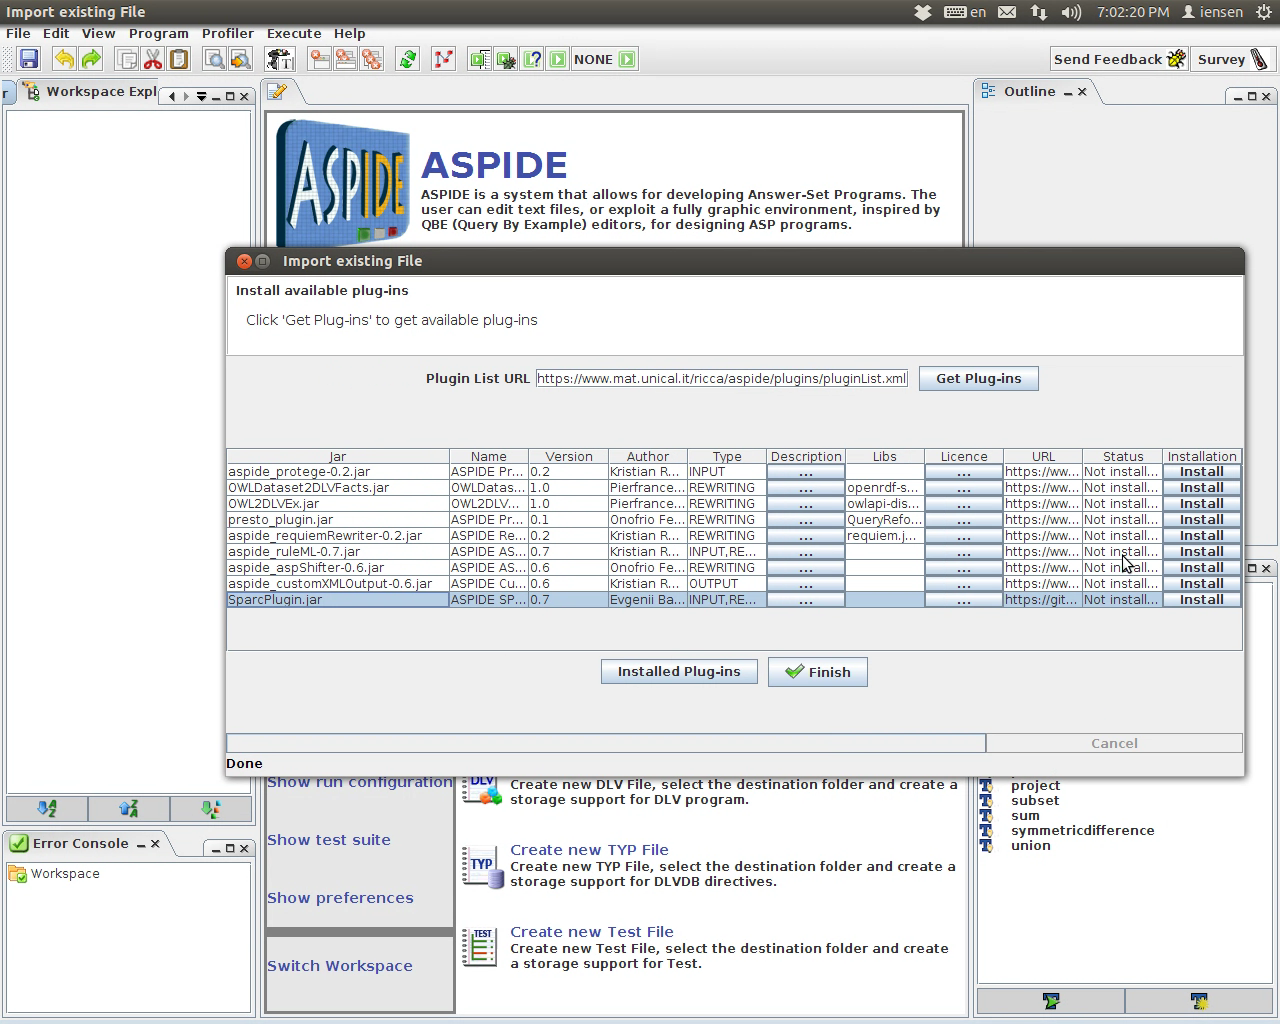
\includegraphics[width=0.9\textwidth]{plugin.png}
\caption{Installing ${\cal SPARC}$ plugin}
\label{fig:plug_install}
\end{figure}

Once the plugin is installed, you can create a source file and start coding (see Fig.\ref{fig:sparc_file}).
You can issue queries and compute answer sets as for usual ASP file.
\begin{figure}[p]
\centering
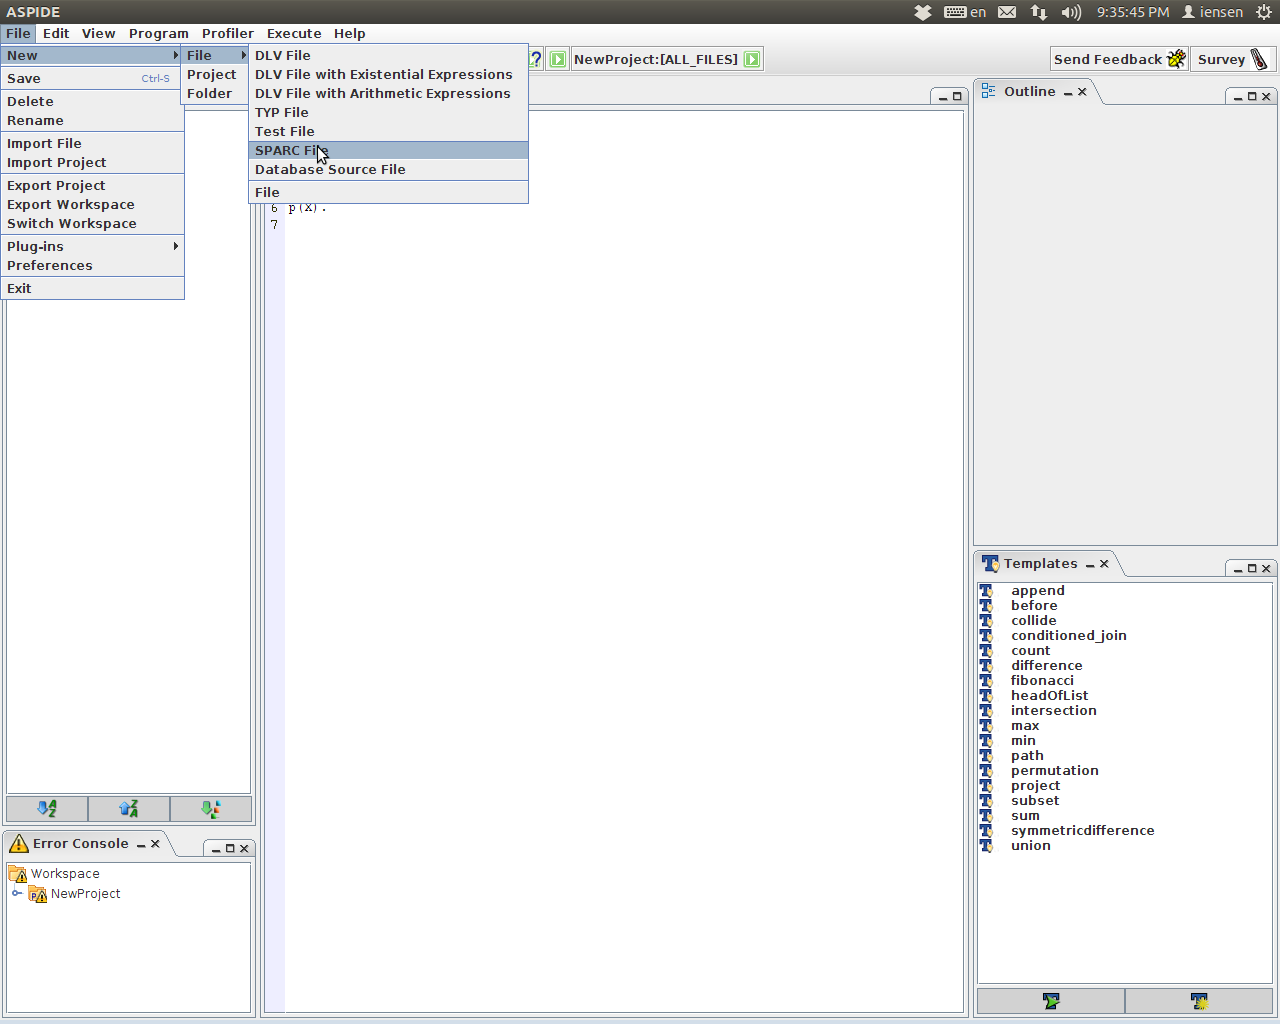
\includegraphics[width=0.9\textwidth]{sparc_file.png}
\caption{Editing  ${\cal SPARC}$ source file}
\label{fig:sparc_file}
\end{figure}
\end{document}